\subsection{Examples of Recommender Systems}
\label{subsec:recommender:examples}

As our solution will combine different recommender systems, we need a short introduction to some of the approaches we will use.
Let us take a closer look at (1) \emph{baseline ratings}, (2) \emph{neighborhood estimation}, (3) \emph{dimensionality reduction}, 
and (4) \emph{network traversal}. This is by no means an exhaustive list, but rather
a quick rundown of common approaches in recommender systems, that we will use in the Chapter \ref{chap:methods}.
See \cite{Adomavicius2005}, \cite{Pazzani2007}, \cite{Schafer2007} or \cite{Bjorkoy2010d} for a more comprehensive exploration of different types of recommenders.
\cite{Segaran2007} gives a good introduction to how RSs are used in practice.

\emph{(1) Baseline ratings} are the simplest family of recommender systems.
These methods compute predictions through varying types of averages of known data.
The data is content-based, and used to compute heuristic predictions.
While simple in nature, these methods are often helpful starting points for more complex systems, or as 
benchmarks for exploring new approaches. 
For example, \citet[p.2]{Koren2008} computes the baselines for items and users, and
use more involved methods to move this starting point in some direction. 
The baseline (predicted relevance) for a user/item pair is given by

\begin{eqsp}
  b_{ui} = \mu + b_u + b_i.
\end{eqsp}

Here, $\mu$ is the average rating across all items and users, 
$b_u$ is the user baseline and 
$b_i$ is the item baseline.
The user and item baselines correspond to how the user's and item's ratings deviate from the norm.
This makes sense as some items may be consistently rated higher than the average, some users may be 
highly critical in their assessments, and so on. \citeauthor{Koren2008} computes these baselines by solving the
least squares problem

\begin{eqsp}
  \min_{b*} = \sum_{(u,i) \in R} (r_{ui} - \mu - b_u - b_i)^2 + \lambda ( \sum_{u} b_u^2 + \sum_{i} b_i^2 ).
\end{eqsp}

This equation finds baselines that fit the given ratings while trying to reduce overfitting
by punishing greater values, as weighted by the $\lambda$ parameter. 
By using baselines instead of simple averages, more complex predictors gain a better starting point,
or in other words, a better average rating.

Another approach based on simple averages is the  \emph{Slope One} family of recommender algorithms. 
As introduced by \cite{Lemire2005}, these algorithms predict unknown ratings based on the average difference in ratings between two items. 
For example, if item $i$ is on average rated $\delta$ points above item $j$, and user $u$ has rated item $j$,
that is, we predict $\hat{r}_{u,i}$ (the estimated rating) to be $r_{u,j} + \delta$, for all the user's ratings that match this pattern,

\begin{eqsp}
  \hat{r}_{u,i} = \frac{\sum_{j \in R_u} \mathrm{ratings}(j) \times (r_{u,j} + \mathrm{\delta}(i,j))}{\sum_{j \in R_u} \mathrm{ratings}(j) }.
\end{eqsp}

Here, $\hat{r}_{ui}$ is the estimated rating, $R_u$ is the items rated by user $u$, $\mathrm{ratings}(i)$ is the number of ratings for item $i$,
and $\mathrm{\delta}(i,j)$ is the average difference in ratings for items $i$ and $j$.
While simplistic, Slope One is computationally effective and produces results comparable to more complex methods \cite[p.5]{Lemire2005}.

\emph{(2) Neighborhood estimation} is at the core of many recommendation systems. 
This is the basic principle behind most collaborative filtering algorithms. 
Unknown ratings are estimated by averaging the ratings of similar items or users, weighted by their similarity.
Neighborhood-based approaches often work in two steps. First, a neighborhood if similar elements is computed.
second, the similarities and connections within this neighborhood is used to produce a prediction.

A common method for computing user similarity is the \emph{Pearson Correlation Coefficient} (PCC) \cite[p.11]{Segaran2007}.
While simple, the PCC compares favorably to more complex approaches, and is often used as a benchmark 
for testing new ideas (e.g. in \citet{Lemire2005, Ujjin, Konstas}).

The PCC is a statistical measure of the correlation between two variables. In our domain, the variables
are two users, and their measurements are the ratings of co-rated items. 
The coefficient produces a value in the range $[-1,1]$ where $1$ signifies perfect correlation (equal ratings),
$0$ for no correlation and $-1$ for a negative correlation.
The negative correlation can signify two users that have diametrically opposing tastes.
We compute PCC by dividing the covariances of the user ratings with their standard deviations:

\begin{eqsp}
  \mathrm{pcc}(u,v) = \frac{cov(R_u, R_v)}{\sigma_{R_u} \sigma_{R_v}}.
\end{eqsp}

When expanding the terms for covariance and standard deviations, 
and using a limited neighborhood size $n$, we get

\begin{eqsp}
  \mathrm{pcc}_{n}(u,v) = 
    \frac{
      \sum_{i \in K}^{n} (R_{ui} - \bar{R_u}) (R_{vi} - \bar{R_v}) }{ 
        \sqrt{ \sum_{i \in K}^{n} (R_{ui} - \bar{R_u})^2 } 
        \sqrt{ \sum_{i \in K}^{n} (R_{vi} - \bar{R_v})^2 }}.
\end{eqsp}

The limited neighborhood size becomes the statistical sampling size, and is a useful
way of placing an upper bound on the complexity of computing a neighborhood.
$n$ does not have to be a stochastic sampling --- it can also be limited by the number of ratings 
the two compared users have in common, the number of ratings each user have, or something similar,
as denoted by $K$ in the formula.

After a neighborhood is determined, it is time to predict the unknown rating.
For Collaborative filtering approaches, we are interested in the similarity of users,
which means averaging the user neighborhood ratings weighted by similarity \cite[p.16]{Segaran2007}:

\begin{eqsp}
  \bar{r}_{ui} = \frac{ \sum_{v \in K(u,i)} \mathrm{sim}(u,v) \times R_{vi} }{ \sum_{v \in K(u,i)} \mathrm{sim}(u,v) }.
\end{eqsp}

Here, $\mathrm{sim}(u,v)$ is the similarity between two users, $K(u,i)$ is the set of users in the neighborhood of $u$ that have rated item $i$.
This is one of the simplest ways of computing a neighborhood-based prediction.
Most systems use more complex estimations. For instance, \cite{Koren2008} 
uses the baseline ratings discussed above instead of plain user and item ratings, to
remove what they call global effects where some users are generous or strict in their 
explicit preferences, and some items are consistently rated differently than the average.

\emph{Content-based} recommenders compute neighborhoods of items instead of users.
The simplest approach is to find items highly rated by the current user, compute the neighborhood 
by finding items similar to these, and produce ratings by weighting the initial rating
with the similarity of the neighboring items.

The PCC is but one of many methods used to compute neighborhoods. 
Other simple measures include the \emph{euclidean distance} \cite[p.10]{Segaran2007},
Spearman's or Kendall Tau rank correlation coefficients \cite[p.30]{Herlocker2004} --- 
variations on the PCC.
Of course, user similarity does not have to rely on ratings. 
If the system has access to detailed user profiles, these can be used
to estimate the similarity of users.
Similarity metrics from the field of \emph{information retrieval} (IR),
such as the \emph{cosine correlation} of rating vectors,
or content-based similarity metrics are applicable,
as we shall see in Section \ref{sec:search}.

\cite{Bell2007a} shows a more sophisticated neighborhood estimation which computes global interpolation weights,
that can be computed simultaneously for all nearest neighbors.
Combinations of different types of neighborhoods are also possible. 
\cite{Ujjin} use a simple euclidean metric to gather a larger neighborhood, which is then refined using a \emph{genetic algorithm}.
Another common way of computing neighborhoods is by reducing the dimensions of the ratings matrix, as we will now describe.

\emph{(3) Dimensionality reduction} is an oft-used technique when creating recommender systems.
The ratings matrix is factored into a set of lower dimension matrices, that can be used to approximate the original matrix.
By reducing the noise in the ratings matrix, and keeping those ratings that contribute to global patterns,
we can identify groups of users, items or combinations that have something in common.
This can then be used to find neighborhoods, compute similarities and estimate unknown ratings.

\emph{Singular Value Decomposition} (SVD) is a common method for such matrix factorization (e.g. \citet[p.5]{Billsus}, \citet{Sun2005}, \citet{Bell2007}).  
This is the same underlying technique used by \emph{latent semantic indexing} in information retrieval \cite[p.44]{Baeza-Yates1999}.
Formally, SVD is the factorization $R = U \Sigma V^{T}$. 
$R$ is an $m \times n$ matrix, in our case the ratings matrix, with $m$ users and $n$ items. 
$U$ is an $m \times m$ factor, $V^{T}$ (the transpose of $V$) is an $n \times n$ factor.
$\Sigma$ is a $m \times n$ diagonal matrix. 
$\Sigma$ is a diagonal matrix, made up of what is called the \emph{singular values} of the original matrix.

The dimensionality reduction can be performed by truncating the factor matrices each to a number of rows or columns, 
where the number is a parameter depending on the current domain and data, called the $rank$ ($r$).
The truncated matrix is $R_r = U_r \Sigma_r V_r^{*}$, where $U_r$ are the first $r$ columns of $U$,
$V_r^{T}$ are the first $r$ rows of $V^{T}$ and $\Sigma_r$ is the top-left $r \times r$ sub-matrix of $\Sigma$.
There are many more complex ways of compressing the matrix than pure truncation, but this is a common way of reducing the factors.
By truncating the factors, we in essence create a higher-level approximation of the original matrix that can identify latent features in the data.
With the factors reduced to $r$ dimensions, the resulting matrices are compressed:

\begin{eqsp}
  \begin{bmatrix}
    { } & { } & { }     & { } & { }\\
    { } & { } & { }     & { } & { }\\
    { } & { } & R_{m,n} & { } & { }\\
    { } & { } & { }     & { } & { }\\
    { } & { } & { }     & { } & { }
  \end{bmatrix} 
  \quad 
  \Rightarrow
  \quad
  \begin{bmatrix}
    { }\\
    { }\\
    U_{m,r}\\
    { }\\
    { }
  \end{bmatrix}
  %\quad
  \begin{bmatrix}
    \Sigma_{r,r}
  \end{bmatrix}
  %\quad
  \begin{bmatrix}
    { } & { } & V_{r,n}^{*} & { } & { }\\
  \end{bmatrix} 
\end{eqsp}

Two important transformations happen in this dimensionality reduction. 
First, ratings that do not contribute to any greater pattern are removed as noise.
Second, ratings that in some way correlate to each other are enhanced, giving more weight to the actual predictive parts of the data.
This means that the reduced factors can for instance identify features that correspond to correlations between items or users.
These features are comparable to the mapping of terms to concepts in LSI.

\begin{figure}[t]
  
\includegraphics[width=\textwidth]{../graphics/compression}
  \caption[SVD Image Compression]{
    SVD Image Compression:
    A variation of using SVD to compress an image, from \cite{Ranade2007}.
    The original image is on the left, and successive images use an increasing number of factors (2, 8 and 30) when performing compression.
    Figure adapted from \citet[p.4]{Ranade2007}.
  }
  \label{fig:svd-image}
\end{figure}

Because SVD can find the most descriptive parts of a matrix, this technique is often used for image compression.
The image we wish to compress is treated as an $N \times M$ matrix, which is run through an SVD factorization.
The factors are truncated, and the result expanded to a matrix that is much simpler to represent
than our original image matrix. As seen in Figure \ref{fig:svd-image}, how close the compressed image resembles the original image
depends on the chosen $rank$, i.e. how many rows and columns we keep during truncation.
A higher rank means less dimensionality reduction and less compression of the image.

The key question for any SVD algorithm is how it performs the factorization,
and which rank the original matrix is reduced to.
Two common factorization methods are the EM and the ALSWR algorithms.
An EM factorizer uses the Expectation-Maximization algorithm to find the factors.
An ALSWR factorizer performs the same factorization with a least-squares approach \citep{Zhou2008}.
The number of features refers to the truncation of the factors in order to reduce the concept-space.
These features then correspond to the number of latent taste categories we wish to identify.
Naturally, different numbers of features will yield different recommenders.
The SVD factorization algorithms are iterative methods, where each iteration
yields more accurate results.

In recommender systems, SVD is used to compress the ratings space into what is sometimes called a \emph{taste space},
where users are mapped to higher-level \emph{taste} categories
(e.g. \citet[p.5]{Ahn2004}, \citet[p.4]{Brand2003} or \citet[p.2]{Liu2006}).
In a taste space,
the collections of individual ratings are reduced to groups of users, items and combinations that have patterns in common.
This reduction makes it easy to find similar users that share some global characteristic.
We can also find similarities between items, clusters of items and user and so on, all based on latent categories
discovered by the automatic identification of patterns in the data.
SVD is then an ingenious way of dealing with the commonly sparse ratings data, by identifying latent correlations and patterns in the data,
which is exactly what we need to predict unknown ratings or connections.

\emph{(4) Network traversal recommenders} refers to estimating predictions by traversing a graph of users and items to provide recommendations.
The connections between nodes can be any type of relation that makes sense to the RS. Examples include linking item and user nodes
based on purchases or explicit ratings, linking user nodes from asymmetrical (directed edges) symmetrical (undirected edges) relations,
or linking items based on some similarity metric.
Recommender systems can use common graph-traversal algorithms to infer unknown connections in this graph.

\cite{Huang2002} used network traversal to create a simple system for recommending books to customers.
Here, edges between items and users correspond to ratings, and edges connecting nodes of the same type
are created by connecting elements that have similarity above a certain threshold. Predictions are generated
by traversing the graph a preset number of steps starting at the current user, and multiplying the weights
of paths leading to the target item (see Figure \ref{fig:book-graphs}).

\begin{figure}[t]
  \centering
  \subfloat[]{\label{fig:graph-layers}
    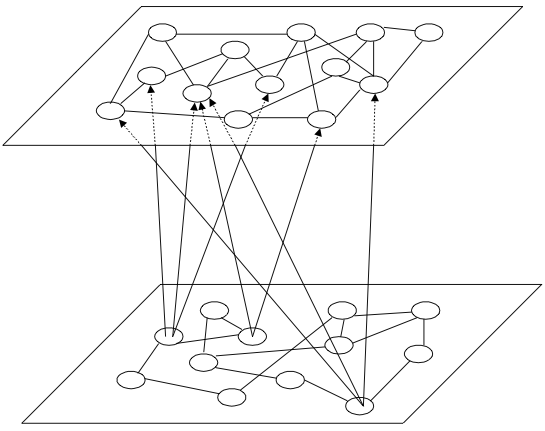
\includegraphics[width=0.5\textwidth]{../graphics/graph-layers}}                
  \subfloat[]{\label{fig:graph-layers-detail}
    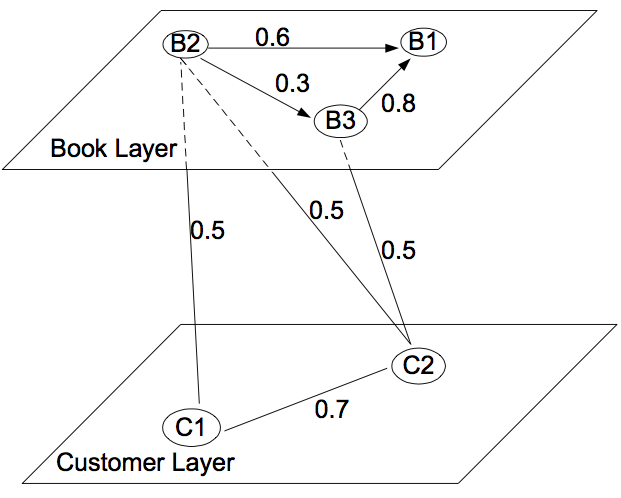
\includegraphics[width=0.5\textwidth]{../graphics/graph-layers-detail}}
  \caption[Example of Network Traversal]{Network Traversal Example: (a) A graph with two kinds of nodes,
    e.g. items and users. (b) A graph with books and customers, where recommendations
    can be made by traversing the weighted connections. Connections between nodes of the same type
    represent similarity, while connections between books and customers represent purchases.
    Figures from \cite{Huang2002}.}
  \label{fig:book-graphs}
\end{figure}
%
The complexity of recommender systems based on networks are only limited by the kinds of relations we can produce.
For example, recommending other users in social networks can easily utilize friend or friend-of-a-friend relations
to find others the current user might be interested in connecting to. Indeed, any relevant similarity metric can be used to
connect nodes of the same type, or nodes of different types.

One variation comes from \cite{Walter2008}, who create a network of \emph{transitive trust} to produce recommendations. Here,
the neighborhood of users is determined by traversing through users connected by a level of trust. 
The trust can for example be a function of how many agreeable results the connection to a user has produced.
Users trust each other's recommendations based on previous experience.

\cite{Konstas} takes yet another approach that measures the similarity between two nodes through their \emph{random walks with restarts} (RWR) technique.
Starting from a node $x$, the RWR algorithm randomly follows a link to a neighboring node. 
In every step, there is a probability $\alpha$ that the algorithm will restart its random walk from the same node, $x$. 
A user-specific column vector $P^{(t)}$ stores the long term probability rates of each node, 
where $P^{(t)}_i$ represents the probability that the random walk at step $t$ is at node $i$. 
$S$ is the column-normalized adjacency-matrix of the graph, i.e. the transition probability table. 
$Q$ is a column vector of zeroes with a value of $1$ at the starting node (that is, $Q_i$ is $1$ when the RWR algorithm starts at node $x$). 
The stationary probabilities of each node, signifying their long term visiting rate, is then given by 

\begin{eqsp}
  P^{(t+1)} = (1 - \alpha)SP^{(t)} + {\alpha}Q.
\end{eqsp}

This algorithm is then run to convergence (within a small delta). Then, the \emph{relatedness} of nodes $x$ and $y$ is given by $P_y$ where $p$ is the user model for the user represented by node $x$.
\citeauthor{Konstas} found that this approach outperformed the PCC, as long as the social networks were an explicit part of the system in question.
The connections between users had to be one actively created by the users to be of such quality and precision that
accurate predictions could be made.

After this whirlwind tour of recommender systems, it is time to look at some closely related topics:
information retrieval and personalized search. This will form the basis for the case study
performed in Chapter \ref{chap:results}.

\clearpage
